

\documentclass{sig-alternate-05-2015}

% Include useful packages
\usepackage{graphicx}
\graphicspath{ {images/} }
\usepackage{float}
\usepackage{subfig}
\usepackage[table,xcdraw]{xcolor}

\newcommand{\todo}{{\\ \huge \color{red} Still need to do this!!!}} % Inserts Todos Statement

\DeclareMathOperator*{\argmin}{argmin} % Argmin
\DeclareMathOperator*{\argmax}{argmax} % Argmax

\begin{document}

% Copyright
\setcopyright{acmcopyright}


\title{A Reimplementation of Online Tracking by Learning Discriminative Saliency Map with Convolutional Neural Network}

\numberofauthors{2} 
\author{
% You can go ahead and credit any number of authors here,
% e.g. one 'row of three' or two rows (consisting of one row of three
% and a second row of one, two or three).
%
% The command \alignauthor (no curly braces needed) should
% precede each author name, affiliation/snail-mail address and
% e-mail address. Additionally, tag each line of
% affiliation/address with \affaddr, and tag the
% e-mail address with \email.
%
% 1st. author
\alignauthor
Aaron Gonzales\\
       \email{gonza647@msu.edu}
% 2nd. author
\alignauthor
Steven MW Hoffman \\
       \email{hoffm470@msu.edu}
}
% There's nothing stopping you putting the seventh, eighth, etc.
% author on the opening page (as the 'third row') but we ask,
% for aesthetic reasons that you place these 'additional authors'
% in the \additional authors block, viz.
\date{25 March 2016}
% Just remember to make sure that the TOTAL number of authors
% is the number that will appear on the first page PLUS the
% number that will appear in the \additionalauthors section.

\maketitle

\begin{figure*}[t]
\centering
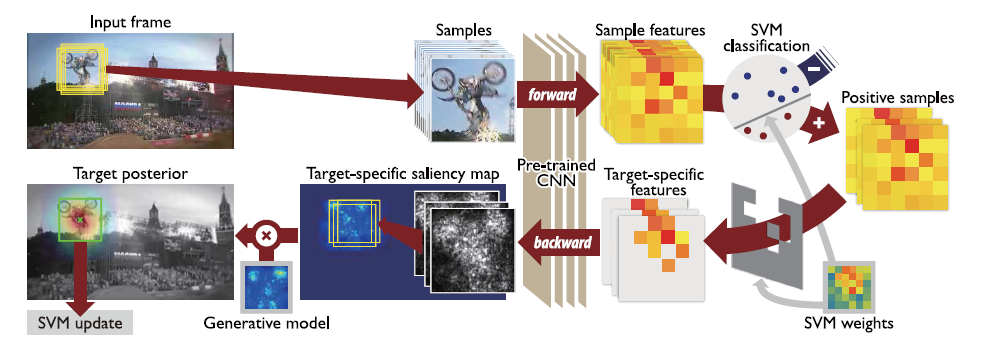
\includegraphics[width=\textwidth]{algorithm}
\caption{A pictoral description of the algorithm described by Hong, et al. in \cite{hong2015online}. Candidate frames are passed through a pre-trained convolutional neural network (CNN) and a feature vector is extracted for each sample from the first fully-connected layer of the CNN. These feature vectors are passed through an SVM, retaining only samples which the SVM believes to contain the target object. The model weights of the SVM are used to determine the target-specific features of each positive sample, which are then back-propagated through the CNN to retrieve a target-specific saliency map. A generative model, produced from previous frames, is convolved with the target-specific saliency map, and the posterior probability that each of the original samples contained the target object is computed.}
\label{fig:algor}
\end{figure*}

\section{Introduction}
We chose to implement our machine learning project with a \textit{deep learning thrust}.
We are basing our project on the work of Hong, et al. \cite{hong2015online}, and our goal is to reproduce their work through the creation of a viable demo.
Hong, et al. propose a novel online tracking scheme for use in applications where tracking an object through frames of a video is desired.
Although there are a large range of potential applications for object tracking software, it is still a difficult problem due to challenges of occlusion, pose variations, illumination changes, fast motion, and background clutter \cite{hong2015online}, and any potential tracking solution must have robust methods to overcome these challenges.
This paper proposes to solve these problems using the combined utility of both a convolutional neural network (CNN) and support vector machine (SVM), wherein a discriminative saliency map is produced and used to calculate the posterior probability of the location of the target in the image.
The object tracking algortihgm by Hong, et al. is described below and is portrayed in Figure~\ref{fig:algor}.

The tracking algorithm proposed by~\cite{hong2015online} begins by first generating a set of sample images, each of which is drawn from candidate bounding boxes near where the target was located in the previous frame.
Each of these sample images is passed through a pre-trained CNN~\cite{jia2014caffe}.
A CNN is used because CNNs have been shown to be very successful at creating image representations useful for object discrimination.
Additionally, CNNs have shown promise in overcoming challenges from many of the current difficulties presented in object tracking, including pose variations, illumination changes, and background clutter.
For each image, the output from \textit{the first fully-connected layer} of the network is extracted and is used as the feature vector describing that image sample.
The image sample feature vector is then given to an SVM which will classify it as either a positive sample, including the object we are tracking, or a negative sample, which does not include the object we are tracking.
In contrast to the CNN, which is learned offline on generic image data not specific to the target, the SVM is learned online using the samples it has seen up to the previous video frame.
This allows the SVM to adapt to different types of objects which the user would like to track.
For each positive sample, the target-specific features are extracted by using those features which corresponded to positive weights in the SVM, setting all other feature values to zero.
The positive weights of the SVM are chosen because they are the weights which correspond to positively identifying a target.
These target-specific features are then backpropagated through the CNN, producing an image containing a saliency map.
A saliency map is created for every positive sample, and these are combined to make a final target-specific saliency map where larger values in the map indicate a larger likelihood that the target is located at that pixel.
Through these means, the target can be segmented out of the image at a near pixel level.
A generative model is then computed to refine the likelihood estimate based on what has been seen in previous frames.
Finally, the posterior probability of each original sample containing the target is calculated, and the bounding box containing the highest posterior is selected as the target location.
With the target successfully found, the algorithm begins anew in the next frame, creating candidate bounding boxes around where it just found the target in the preceding frame.

\section{Related Work}
The problem of object tracking in video is a large domain, so we will restrict our discussion here to a few works which also attempted to use CNNs to perform tracking, as these are most relevant to the paper we have chosen by Hong, et al. \cite{hong2015online}.
We also highlight how the approach proposed by Hong, et al. differs from these approaches, making it a novel work.

\cite{fan2010human} utilizes a CNN for tracking; however they use an offline trained CNN. They also require a separate class-specific network to track various other objects. Hong, et al \cite{hong2015online}, in contrast, proposes using a pre-trained CNN used for large scale image classification which is trained on generic image data. An online trained SVM is then used in conjunction with the CNN by Hong, et al. to learn the target specific information.

\cite{NIPS2013_5192} also uses a pre-trained network where a stacked denoising autoencoder is trained using a large number of images to learn generic image features. However, as this network is trained on small grey images, its representation power is limited.

\cite{7362006} proposed a target-specific CNN for tracking, where the CNN is trained online. However, this network is shallow in comparison with the deep CNN proposed by \cite{hong2015online}, and as such does not take advantage of the rich information a deep CNN provides.

In addition to the novelties described above, the tracking method proposed by \cite{hong2015online} differs from all three of the above papers in a few important ways.
First, it uses an online trained SVM with the offline trained CNN in order to adapt the tracking to whatever type of object the algorithm happens to be presented with.
Secondly, it uses saliency maps to find the precise location of the tracked object.

\section{Dataset Description}
Following the form of Hong, et al.~\cite{hong2015online}, we tested the tracking algorithm against video sequences from the Tracker Benchmark v1.0 dataset~\cite{wu2013online}. 
This dataset contains 50 testing sequences, i.e. videos containing a specific object to track, all of which vary in video length.
These sequences present a variety of tracking challenges such as illumination variation, deformation, motion blur, background clutter, etc, which can be seen in Table~\ref{tab:vid-attr}.
In addition to these visual challenges, objects of interest vary from humans, to vehicles, to animals, and to various inanimate objects. 
Each of these sequences contain ground truth text files which contain bounding box information for objects of interest at each frame of the video. 
Some of the videos contain multiple objects of interest and as a result come with multiple ground truth files. 
We will analyze our tracking results on these videos qualitatively.
Video frames from a selection of these testing sequences is shown in Figure~\ref{fig:tracker-benchmark}.


% http://www.tablesgenerator.com/ was used to create this table
\begin{table}[]
\centering
\caption{Various video attributes contained within the Tracker Benchmark v1.0 dataset which make objects harder to track in the video. Each of the 50 test videos is annotated with the attributes which that video contains~\cite{wu2013online}.}
\label{tab:vid-attr}
\begin{tabular}{|
>{\columncolor[HTML]{C0C0C0}}c |p{6cm}|}
\hline
\multicolumn{1}{|l|}{\cellcolor[HTML]{C0C0C0}Video Attribute} & \cellcolor[HTML]{C0C0C0}Description                                                                                                                     \\ \hline
IV                                                            & \textit{Illumination Variation}: the illumination in the target region is significantly changed.                                                                 \\ \hline
SV                                                            & \textit{Scale Variation}: the ratio of the bounding boxes of the first frame and,the current frame is out of the range {[}1/ts, ts{]}, ts \textgreater 1 (ts=2). \\ \hline
OCC                                                           & \textit{Occlusion}: the target is partially or fully occluded.                                                                                                   \\ \hline
DEF                                                           & \textit{Deformation}: non-rigid object deformation.                                                                                                              \\ \hline
MB                                                            & \textit{Motion Blur}: the target region is blurred due to the motion of target or camera.                                                                        \\ \hline
FM                                                            & \textit{Fast Motion}: the motion of the ground truth is larger than tm pixels (tm=20).                                                                           \\ \hline
IPR                                                           & \textit{In-Plane Rotation}: the target rotates in the image plane.                                                                                               \\ \hline
OPR                                                           & \textit{Out-of-Plane Rotation}: the target rotates out of the image plane.                                                                                       \\ \hline
OV                                                            & \textit{Out-of-View}: some portion of the target leaves the view.                                                                                                \\ \hline
BC                                                            & \textit{Background Clutters}: the background near the target has the similar color or texture as the target.                                                     \\ \hline
LR                                                            & \textit{Low Resolution}: the number of pixels inside the ground-truth bounding box is less than tr (tr =400).                                                    \\ \hline
\end{tabular}
\end{table}

\begin{figure}[h]
\begin{tabular}{cc}
\subfloat[Deer: MB, FM, IPR, BC, LR]{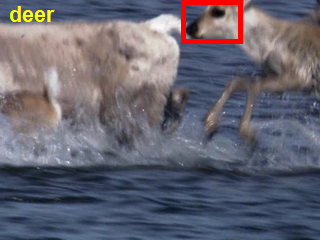
\includegraphics[width = 1.5in]{Deer-ex}}&
\subfloat[MountainBike: IPR, OPR, BC]{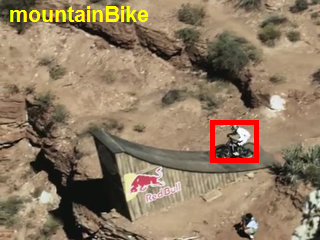
\includegraphics[width = 1.5in]{MountainBike-ex}} \\
\subfloat[Tiger1: IV, OCC, DEF, MB, FM, IPR, OPR]{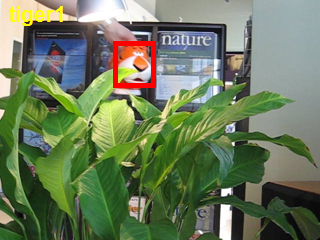
\includegraphics[width = 1.5in]{Tiger1-ex}}&
\subfloat[Walking: SV, OCC, DEF]{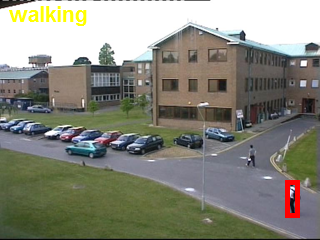
\includegraphics[width = 1.5in]{Walking-ex}} \\
\end{tabular}
\centering
\caption{Video frames from sample sequences in the Tracker Benchmark v1.0 dataset along with bounding boxes drawn around the target object~\cite{wu2013online}. The video attributes are also listed for each shown video.}
\label{fig:tracker-benchmark}
\end{figure}

\section{Tracking Algorithm}
In the introduction, we provided a brief overview of the tracking algorithm proposed by Hong, et al.~\cite{hong2015online}, which we have implemented for our project.
In this section, we will go into more detail describing this algorithm and how we have implemented it.
All of the code for this project was written in Matlab and was executed on both Matlab 2014b and Matlab 2015b.
Note that Figure~\ref{fig:algor} provides a nice pictorial overview of the algorithm.

\subsection{Generating Candidate Sample Patches}
In order to search for the target object in the current frame, candidate sample patches need to be generated, i.e. small portions of the image frame cropped to the size of the target object's initial ground-truth bounding box.
The rest of the tracking algorithm will then be focused on choosing the candidate sample patch, which we will also call a sample or a bounding box, that has the maximum posterior probability of containing the target. 
To generate candidate samples, we first let the bounding box containing the target in the previous frame be a candidate sample for the current frame.
Note that our algorithm will always use the ground truth bounding box provided with the dataset for at least the first frame, beginning tracking with the next frame; this ensures there will always be a bounding box from a previous frame for our algorithm to draw on and it allows us to easily specify which object the algorithm should track in a video by placing the initial bounding box over that object.
We then generate 120 additional samples by drawing from a normal distribution defined by $x_i \sim \mathcal{N}(x_{t-1}^*,\sqrt{wh}/2)$, where $w$ and $h$ denote the width and height of the target bounding box in the initial frame, $x_{t-1}^*$ is the location of the target in the previous frame, and $x_{i}$ is the $i$th sample generated at frame $t$, the current frame. 
This is the same procedure as used by~\cite{hong2015online}, and it is based on the assumption that the most likely locations for the object are distributed around the location of the object in the previous frame.
An example of some of these samples is shown in Figure~\ref{fig:patches}.

\begin{figure}[h]
\centering
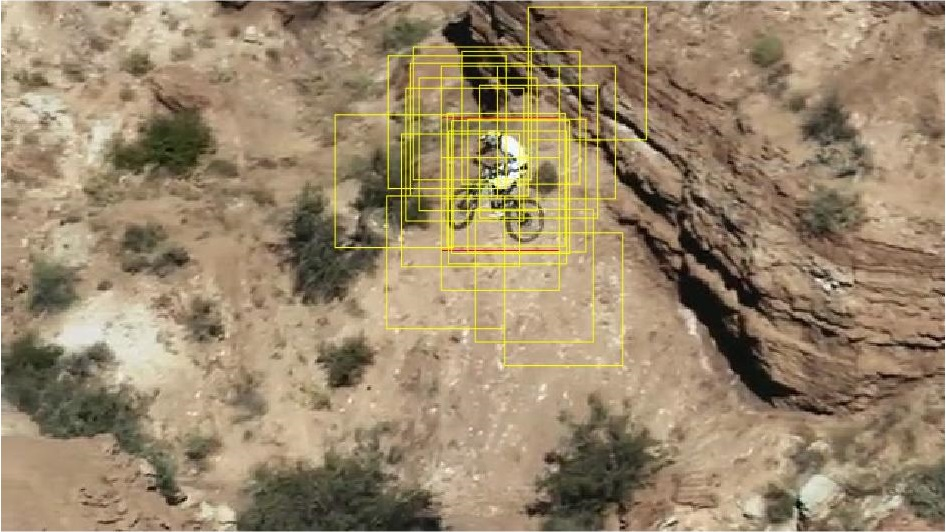
\includegraphics[width = 3in]{samples}
\caption{The location of the target from the previous frame (red box) and the normally sampled candidate patches (yellow boxes) for a biker from the video tracking dataset~\cite{wu2013online}.}
\label{fig:patches}
\end{figure}

\subsection{Computing Sample Features with a CNN}
For the next step of the algorithm, a CNN is used to transform each sample patch into a sample feature vector.
The CNN used should be pre-trained on a dataset for generic object detection in images; this is because CNNs trained for such a task have been known to create transformed representations of images useful for object discrimination~\cite{krizhevsky2012imagenet}.
Each candidate sample is passed through the CNN, and the output of the CNN's first fully-connected layer is used as the feature vector representing that sample.

The original algorithm by Hong, et al.~\cite{hong2015online} used the Caffe Model Zoo implementation of the pre-trained \textit{R-CNN} created by Girshick, et al.~\cite{girshick2016region} to create their sample feature vectors.
However,~\cite{hong2015online} specified in their paper that CNN models other than Girshick's R-CNN may also be used for similar results.
Thus, to circumvent the large amount of time needed to install Caffe, we decided to instead use MatConvNet~\cite{vedaldi2015matconvnet}, a CNN toolkit for Matlab with a simple installation process.
MatConvNet provides several pre-trained CNNs, and we decided to use \textit{VGG-F}, a CNN that has achieved state-of-the-art performance on the ImageNet object recognition database~\cite{chatfield2014return}.

\subsection{Using an SVM to Find Target-Specific Features from Sample Features}
Online SVM code has been acquired from Cauwenberghs, et al.~\cite{cauwenberghs2001incremental}. 
\todo

\subsection{Computing Target-Specific Saliency Maps}
Once the target-specific features are found for the positive samples, a class-specific saliency map needs to be generated for each of these samples, using the process detailed in~\cite{simonyan2013deep}.
These class-specific saliency maps will then be used to generate a target-specific saliency map, which will be used to find the likelihood of each pixel containing the target.
To compute the class-specific saliency map from the target-specific features of a sample, we first have to insert the target-specific features into the first fully-connected layer of the pre-trained CNN.
After doing this, the features are back-propagated through the CNN back to the input layer of the network.
The data retrieved from the input layer of the net is of the same size as the original samples, that is of size H x W x C, where H = the height of the target bounding box in the initial frame, W = the width of the target bounding box in the initial frame, and C = the number of color channels in the frames of the video.
If C $\neq 1$, then the resultant data is compressed to a single channel by taking the maximum absolute value across the C channels at every pixel.
This produces a class-specific saliency map for each one of the positive samples.
An example class-specific saliency map is shown in Figure~\ref{fig:saliency}.

\begin{figure}[h]
\begin{tabular}{cc}
\subfloat[Positive Sample]{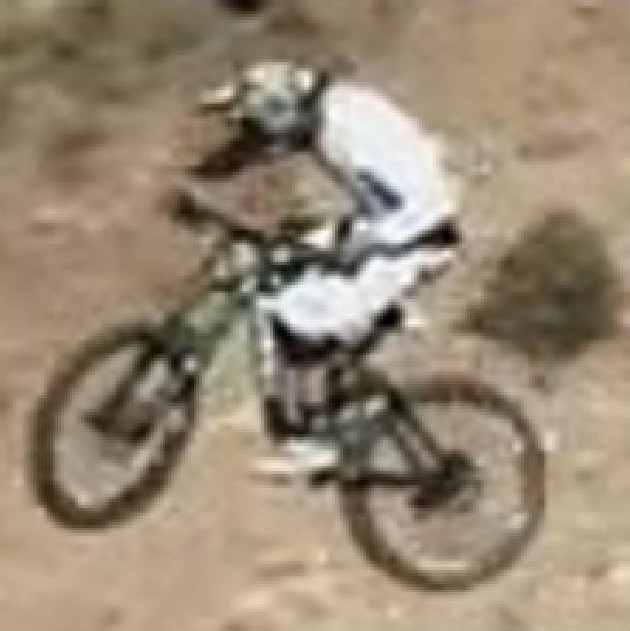
\includegraphics[width = 1.5in]{bike}}&
\subfloat[Class-Specific Saliency Map]{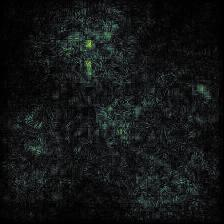
\includegraphics[width = 1.5in]{bike_saliency}}
\end{tabular}
\centering
\caption{The class-specific saliency map produced from a positive candidate sample patch. Note that the regions in the saliency map that have the highest magnitude correspond to pixel locations that contain the target object.}
\label{fig:saliency}
\end{figure}

Once a class-specific saliency map is generated for each positive sample, their data is aggregated into a single target-specific saliency map.
This is done by first zero-padding each class-specific saliency map to the size of the original video frame, taking into account the location from which its corresponding candidate sample patch was cropped from the video frame.
A target-specific saliency map is then generated by taking the maximum value across all the zero-padded class-specific saliency maps at each pixel location.
This produces a single target-specific saliency map that has the same width and height as the original video frame.
An example target-specific saliency map can be seen in Figure~\ref{fig:target-saliency}.

\begin{figure}[h]
\begin{tabular}{c}
\subfloat[Original Video Frame]{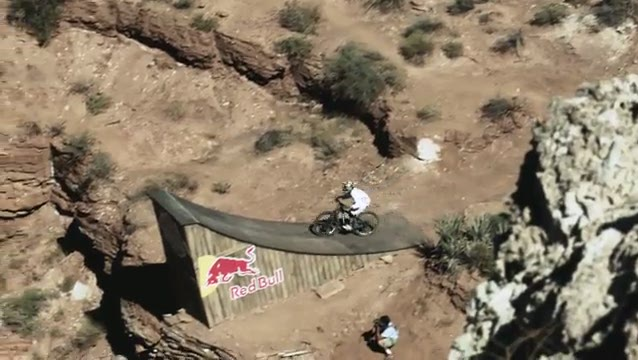
\includegraphics[width = 2.5in]{original_frame}} \\
\subfloat[Target-Specific Saliency Map]{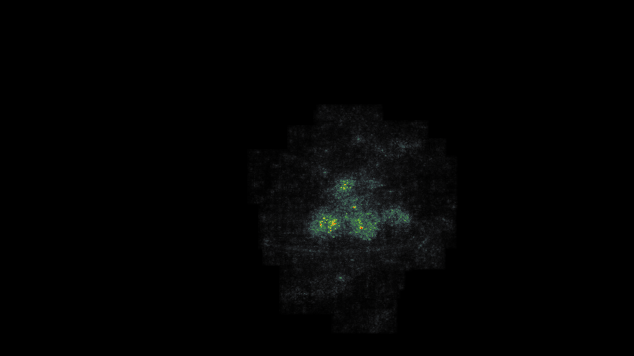
\includegraphics[width = 2.5in]{target_specific_saliency_map}} \\
\subfloat[Target-Specific Saliency Map Overlayed onto Video Frame]{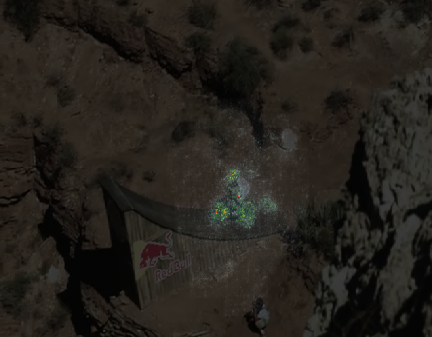
\includegraphics[width = 2.0in]{tssm_overlay}} \\
\end{tabular}
\centering
\caption{The target-specific saliency map produced from all the positive candidate sample patches. Note that the regions in the saliency map that have the highest magnitude correspond to pixel locations that contain the target object.}
\label{fig:target-saliency}
\end{figure}

As noted in~\cite{hong2015online}, back-propagating the features through the CNN is equivalent to taking the derivative of the feature vector in respect to the change in the image.
This means that large values in the saliency maps (produced from back-propagation) indicate those pixel locations where changing the pixel value will most drastically affect the object classification of the CNN (which is determined by the feature vector).
Intuitively, foreground pixels are those that change the CNN object classification the most because the object classification should ideally not be affected by the background pixels.
Thus, the saliency maps capture the likelihood of a pixel being part of the foreground.
Furthermore, because the target-specific features are only produced for the samples which the SVM determined contained the target, this means it is likely that these foreground pixels will be pixels containing the target object.
Removing the features corresponding to non-positive weights further helps to ensure this.
Thus the saliency maps can be used to provide a pixel-wise segmentation of the target object in the frame, as can be seen in Figure~\ref{fig:saliency} and Figure~\ref{fig:target-saliency}.

\subsection{Localizing the Target with Target-Specific Saliency Map}
Given the target-specific saliency map, we wish to locate the target in the video frame.
Hong, et al accomplish this in their algorithm through a process they refer to as \textit{sequential Bayesian filtering}~\cite{hong2015online}.
Let $M_t$ represent the target-specific saliency map at the current frame, frame $t$, and allow $x_t$ to represent one of the candidate sample patches from this frame.
Sequential Bayesian filtering then attempts to compute the \textit{posterior probability} $p(x_t|M_{1:t})$ of each candidate $x_t$ containing the target, given by
\begin{equation}
\label{eq:posterior}
p(x_t|M_{1:t}) \propto p(M_t |x_t)p(x_t|M_{1:t-1})
\end{equation}
where $p(M_t |x_t)$ represents the likelihood of the sample and $p(x_t|M_{1:t-1})$ represents the prior of the sample.
The candidate sample patch with the highest posterior is then selected as the bounding box that contains the target in the current frame $x_t^*$.
The algorithm will then continue by moving to the next frame, repeating the algorithm until all frames have been analyzed.

\subsubsection{Computing the Likelihood with the Generative Model}
In order to determine the likelihood of a candidate sample, a generative model $H_t$ is first computed.
This generative model is computed using the target-specific saliency maps of the $m$ preceding frames where $m$ is a constant, scalar value, set to $m = 30$ in~\cite{hong2015online}.
Let $x_k^*$ indicate the bounding box of the located target in frame $k$ and $M_k(x^*_k)$ denote the target-specific saliency map at frame $k$ cropped to the bounding box $x^*_k$.
Hence, $M_k(x^*_k)$ shows how the target appeared in the saliency map at frame $k$.
The generative model is then computed by simply finding the average appearance of the target in the last $m$ frames:
\begin{equation}
H_t = \frac{1}{m} \sum_{k=t-m}^{t-1} M_k(x^*_k)
\end{equation}
The likelihood of a candidate patch $x_t$ is then found by convolving the generative model $H_t$ with the current saliency map cropped to the candidate patch $M_t(x_t)$, as follows:
\begin{equation}
p(M_t|x_t) \propto H_t \otimes M_t(x_t)
\end{equation}
where $\otimes$ represents the convolution operator.
The likelihood of each candidate sample patch is then found in this way, using the same generative model for all patches.

\subsubsection{Computing the Prior}
To find the prior $p(x_t|M_{1:t-1})$ of a candidate patch $x_t$, both the location of this bounding box and the posterior distribution from the previous frame is considered.
The prior is computed through the following formula:
\begin{equation}
\label{eq:prior}
p(x_t|M_{1:t-1}) = \int p(x_t|x_{t-1}) p(x_{t-1}|M_{1:t-1}) dx_{t-1}
\end{equation}
This equation shows that a candidate's prior is the sum over all the candidates from the previous frame $x_{t-1}$ of a location-based probability $p(x_t|x_{t-1})$ weighted by the previous frame's candidates' posterior probabilities $p(x_t|M_{1:t-1})$.
The posterior probabilities were already calculated during the last iteration of the algorithm; the location-based probability, however, needs to be calculated.
To do this, the mean $\mu_t$ and covariance $\Sigma_t$ of the locations of the positive samples from the current frame are calculated.
Then, the amount $d_t$ that the target object has moved between frames $t-1$ and $t$ is estimated using the following formula:
\begin{equation}
d_t = \mu_t - x^*_{t-1}
\end{equation}
where $x^*_{t-1}$ is the estimated location of the target object in the previous frame.
It is then assumed that the the probability of the target object moving to a location is normally distributed around a mean of the distance vector $d_t$ with covariance $\Sigma_t$.
Thus the location-based probability of a candidate sample in relation to a candidate sample from the previous frame is found by:
\begin{equation}
\label{eq:loc-based-prob-prior}
p(x_t|x_{t-1}) = \mathcal{N}(x_t-x_{t-1}; d_t ; \Sigma_t)
\end{equation}
Plugging this into Equation~\ref{eq:prior} allows the prior for each candidate sample in the current frame to be computed.

\subsubsection{Computing the Target Posterior}
After computing the likelihoods and priors, the target posterior $p(x_t|M_{1:t})$ for a candidate sample patch can then be computed by using Equation~\ref{eq:posterior}.
The location of the target in the current frame $x_t^*$ is then set as the candidate patch with the highest posterior according to the following equation:
\begin{equation}
x_t^* = \argmax_{x_t} p(x_t|M_{1:t})
\end{equation}
Having found the target in the current frame, the algorithm then has the option to update the training of the SVM, as detailed Section~\ref{sec:training-svm}.
After this, the algorithm begins its next iteration by searching for the object in the next frame, $t+1$, starting by generating new candidate sample patches around $x_t^*$.

Note that in practice, we found that if the target object moved too much between a pair of frames, the prior probability, which gives preference to bounding boxes that have not moved very much, would prevent the algorithm from selecting candidate sample containing the target object.
Therefore, we found that the algorithm produces more accurate and smooth results when the prior is not used to calculate the posterior, using a modified posterior $p(x_t|M_{1:t})'$ such that
\begin{equation}
\label{eq:posterior-mod}
p(x_t|M_{1:t})' \propto p(M_t |x_t)
\end{equation}
Because of this, the majority of our reported results do not use the prior to calculate the posterior.
This is discussed further when discussing the results below.

\subsection{Training the SVM}
\label{sec:training-svm} % Keep this label in the section describing the SVM
-
\todo

\section{Results}
We ran our algorithm on many different videos from the Tracker Benchmark v1.0 dataset~\cite{wu2013online} and analyzed the resulting videos qualitatively.
Some of these results can be found on our GitHub page here: \verb!https://github.com/msu-ml/16spr_cao_gonzales_hoffman/tree/master/results!.
In the following sections, we present and analyze some of these results.

\subsection{How the Prior and the SVM Affect the Tracking}
Early on in testing our algorithm, we decided to analyze how the SVM affects the tracking algorithm and also how using the prior probability in determining the posteriors, i.e. using Equation~\ref{eq:posterior}, affects the algorithm in comparison to not using the prior, i.e. using Equation~\ref{eq:posterior-mod}.
This section presents and discusses some of these results.
The video sequences referred to in this section can be viewed at the following location on our GitHub page: \verb!https://github.com/msu-ml/16spr_cao_gonzales_hoffman/tree/master/results/Affects-of-Prior-and-SVM-Results!.

The first test we decided to perform was to compare using the prior and not using the prior.
We first tested this without the SVM because we had not yet implemented the SVM.
The reason we decided to test the affect of the prior is because we noticed that for some video sequences, the target object would move a relatively large distance in between frames, i.e. the object was moving fast, and our tracking algorithm was not following the object when this happened.
For example, a few frames from the \textit{Deer} video sequence where this fast object movement occurs are shown in Figure~\ref{fig:deer-p-ns}.

\begin{figure}[h]
\begin{tabular}{c}
\subfloat[frame = 2]{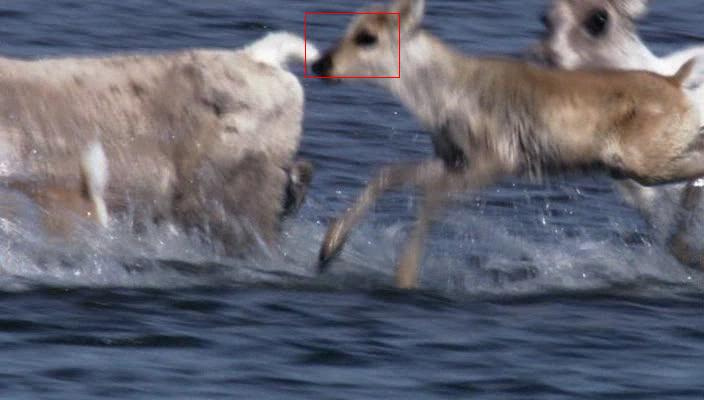
\includegraphics[width = 2.5in]{Deer-P-NS-0002}} \\
\subfloat[frame = 3]{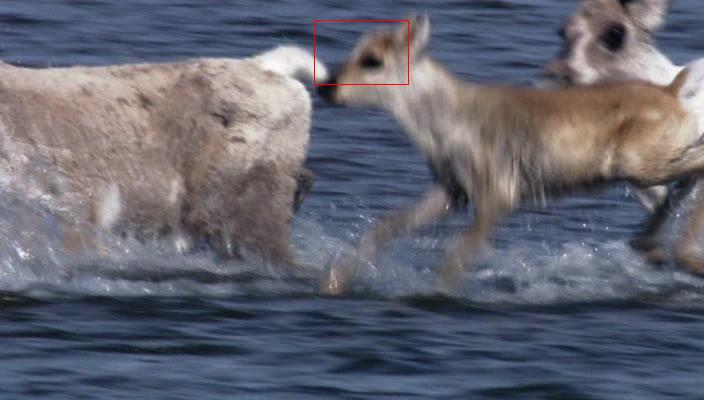
\includegraphics[width = 2.5in]{Deer-P-NS-0003}} \\
\subfloat[frame = 4]{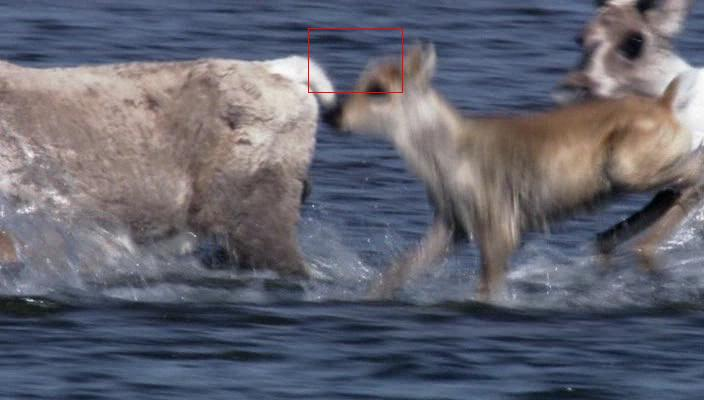
\includegraphics[width = 2.5in]{Deer-P-NS-0004}} \\
\end{tabular}
\centering
\caption{A video tracking sequence showing fast object movement, which caused the algorithm to fail. The prior was used and an SVM was not used in this sequence.}
\label{fig:deer-p-ns}
\end{figure}

We hypothesized that this failure was due to the use of the prior in calculating the posterior probability in Equation~\ref{eq:posterior}.
The prior probability algorithm contains a component that functions as a location-based probability (see Equation~\ref{eq:loc-based-prob-prior}); this means that the prior probability for a sample will be higher for candidate samples that are close to the target object in the previous frame.
Thus, when the target object moves a large distance between frames, the candidate sample that corresponds to the moved target will have a \textit{low} prior since it is far from where the target was in the previous frame.
Our hypothesis then was that this caused the candidate samples to occasionally have such a low posterior probability that other candidate samples, not containing the target, actually had a larger posterior probability and were selected by our algorithm as containing the target.

To test this hypothesis, we ran the same \textit{Deer} sequence using the modified posterior probability (Equation~\ref{eq:posterior-mod}) that does not take into account the prior probabilities.
A few resulting frames are shown in Figure~\ref{fig:deer-np-ns}.
As can be seen from these results, the tracking algorithm performed significantly better overall when the prior was not used in comparison to when the prior was used.
We also performed this test on a few other sequences, including the \textit{MountainBike} sequence, and found the same pattern to be true.
This empirically confirmed our hypothesis that the prior probability was causing errors for fast-moving objects.

\begin{figure}[h]
\begin{tabular}{c}
\subfloat[frame = 2]{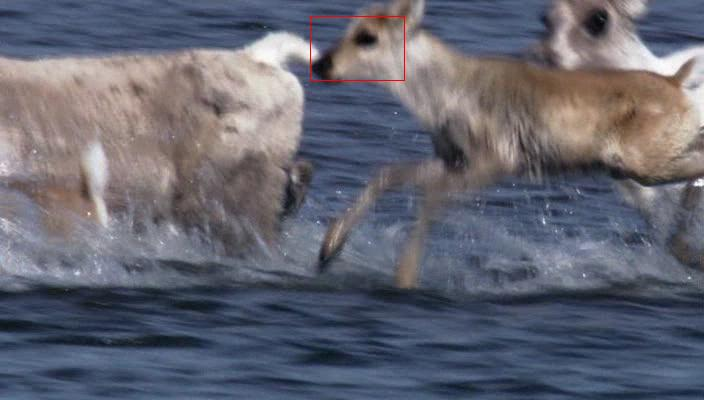
\includegraphics[width = 2.5in]{Deer-NP-NS-0002}} \\
\subfloat[frame = 3]{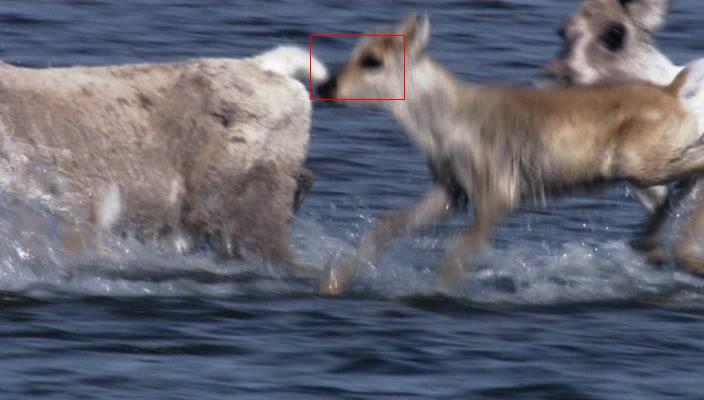
\includegraphics[width = 2.5in]{Deer-NP-NS-0003}} \\
\subfloat[frame = 4]{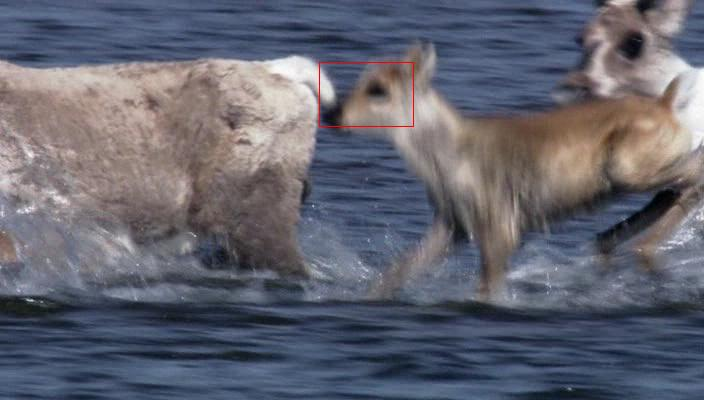
\includegraphics[width = 2.5in]{Deer-NP-NS-0004}} \\
\end{tabular}
\centering
\caption{A video tracking sequence showing fast object movement, which the algorithm was able to account for. The prior was not used and an SVM was not used in this sequence. Notice the performance increase compared to when a prior was used in Figure~\ref{fig:deer-p-ns}.}
\label{fig:deer-np-ns}
\end{figure}

Having tested how the prior affects the tracking \textit{without} using an SVM, we decided that our next test would be to see how including the SVM would affect the tracking.
We noticed that without the SVM, the tracking would occasionally loose the target, either to track another object or thinking that the background was the target object.
This is seen in Figure~\ref{fig:deer-np-ns-2}.
Including the SVM would allow the algorithm to remember what the target object looks like and, we hypothesized, increase the accuracy.
After performing several tests including the SVM, we noted that overall, the SVM did significantly improve the tracking accuracy, as expected.
An example of this is seen in Figure~\ref{fig:deer-np-s}, where the SVM helped the algorithm to continue tracking the correct deer through a few problem frames.
We also performed additional tests that showed that using the SVM \textit{with} the prior was able to perform better in some instances than when neither the SVM nor the prior were used, and these results are shown on our GitHub page.

\begin{figure}[h]
\begin{tabular}{c}
\subfloat[frame = 43]{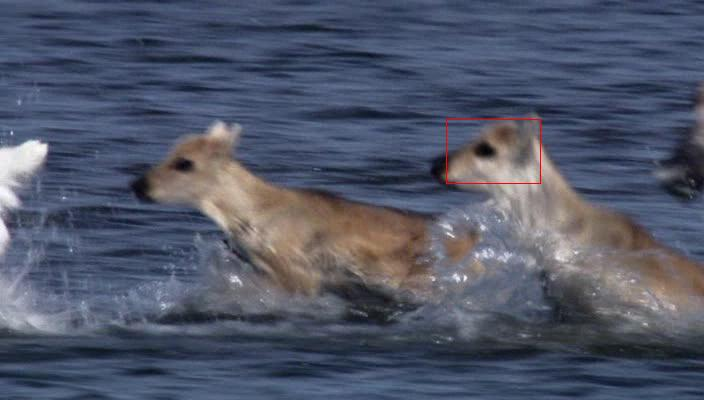
\includegraphics[width = 2.5in]{Deer-NP-NS-0043}} \\
\subfloat[frame = 44]{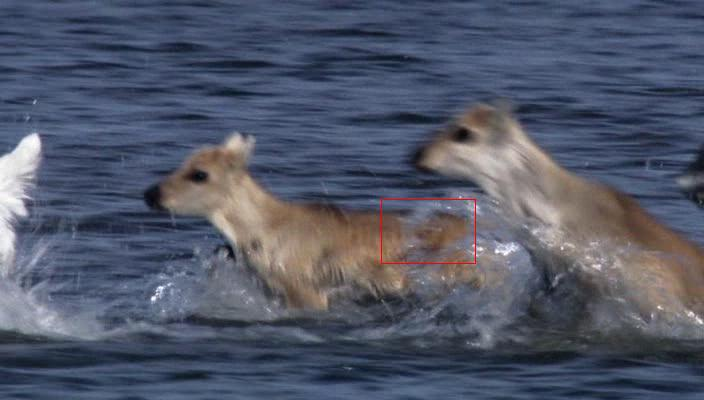
\includegraphics[width = 2.5in]{Deer-NP-NS-0044}} \\
\subfloat[frame = 45]{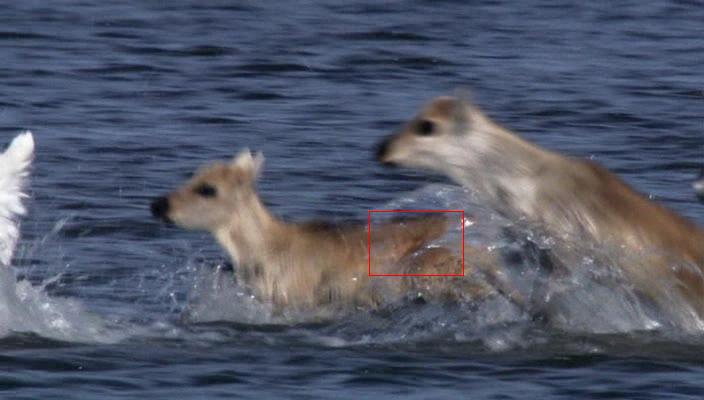
\includegraphics[width = 2.5in]{Deer-NP-NS-0045}} \\
\end{tabular}
\centering
\caption{A video tracking sequence showing the tracking algorithm beginning to track a different object. The prior was not used and an SVM was not used in this sequence.}
\label{fig:deer-np-ns-2}
\end{figure}

\begin{figure}[h]
\begin{tabular}{c}
\subfloat[frame = 43]{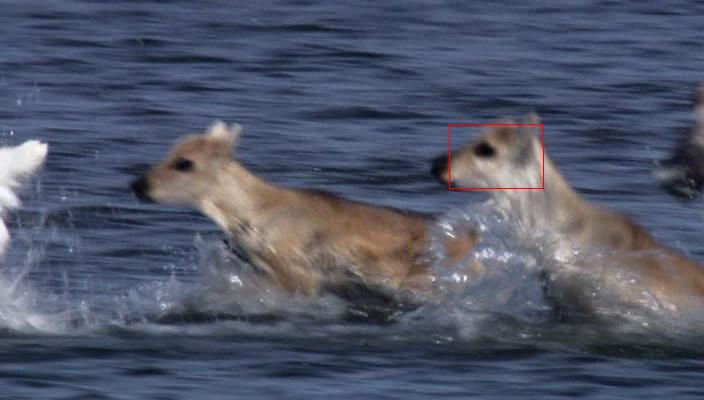
\includegraphics[width = 2.5in]{Deer-NP-S-0043}} \\
\subfloat[frame = 44]{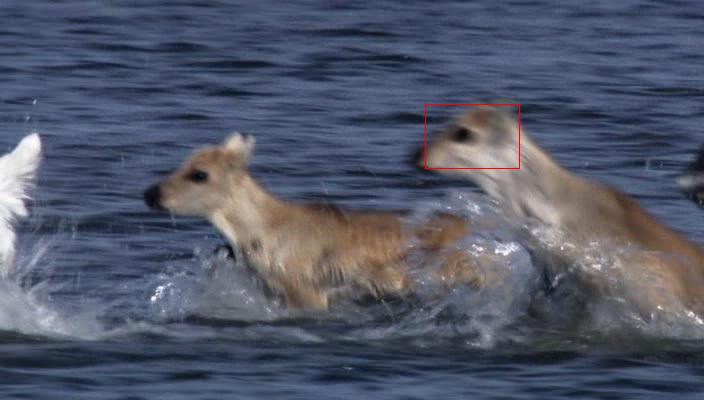
\includegraphics[width = 2.5in]{Deer-NP-S-0044}} \\
\subfloat[frame = 45]{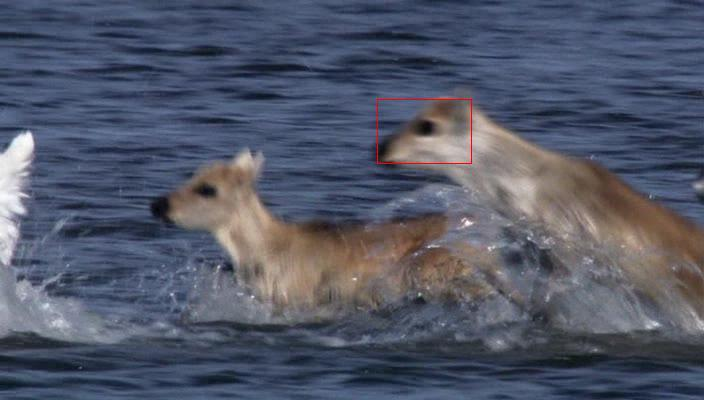
\includegraphics[width = 2.5in]{Deer-NP-S-0045}} \\
\end{tabular}
\centering
\caption{A video tracking sequence showing the tracking algorithm correctly tracking the target object. The prior was not used and an SVM was used in this sequence. Notice the performance increase compared to when an SVM was not used in Figure~\ref{fig:deer-np-ns-2}.}
\label{fig:deer-np-s}
\end{figure}

After all of these tests, we determined that our tracking algorithm performed best when we used the SVM but did not use the prior.
Therefore, the rest of the results shown here use this configuration.

\subsection{Modifying the SVM Training to Improve Tracking}
-
\todo

\subsection{How Object Scale Affects the Tracking}
When testing our algorithm, we noticed that the algorithm has trouble tracking an object when the size, or scale, of the object changes between frames.
This often happens when the target object comes closer to or goes farther away from the camera.
Some examples of our algorithm failing from what we believe are scaling issues are shown in Figure~\ref{fig:scaling1} and Figure~\ref{fig:scaling2}.
The complete video sequences can be found on our GitHub page at \verb!https://github.com/msu-ml/16spr_cao_gonzales_hoffman/tree/master/results/! 

\noindent{\verb!Scale-Variation-Results!.}
Unfortunately, the scaling issue is a problem inherent in the algorithm design by Hong, et al.
This is because the algorithm assumes that the target object's bounding box stays constant for all the frames.
While the algorithm could be modified to check for growing or shrinking bounding boxes, time constraints prevented us from adding this to our code.
This is one task we wish to work on in the future.
As it turns out, many of the tracking errors we have had so far can be attributed to variations in scale.

\begin{figure}[h]
\begin{tabular}{c}
\subfloat[frame = 1]{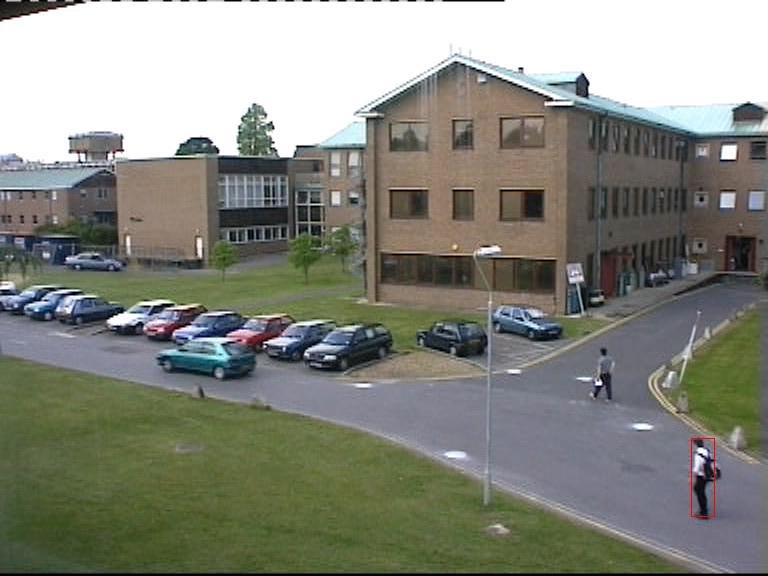
\includegraphics[width = 2.5in]{Walking-0001}} \\
\subfloat[frame = 207]{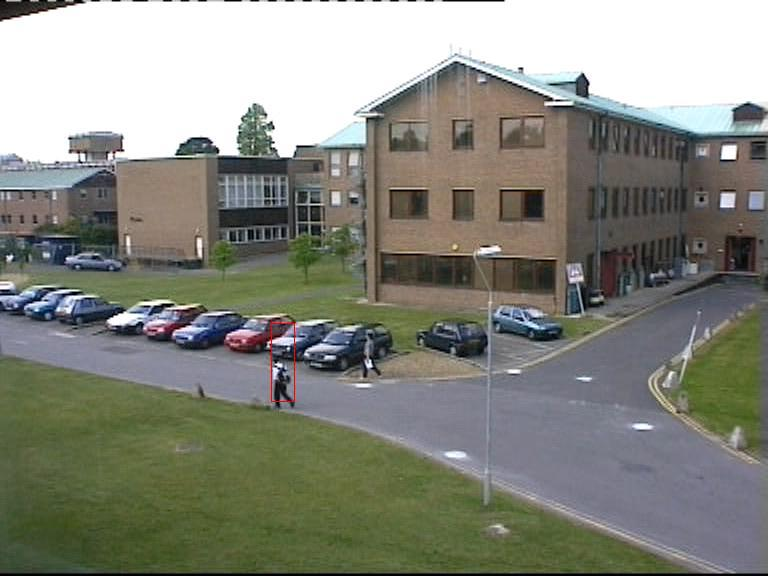
\includegraphics[width = 2.5in]{Walking-0207}} \\
\subfloat[frame = 217]{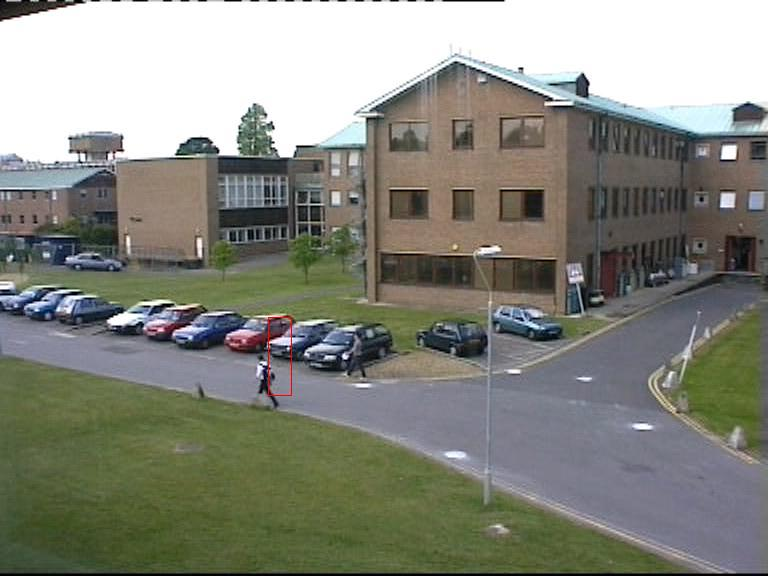
\includegraphics[width = 2.5in]{Walking-0217}} \\
\end{tabular}
\centering
\caption{A video tracking sequence showing the tracking algorithm failing to account for changes in scale. Notice that by frame 217, the target object had shrunken so much that the tracking algorithm no longer recognized it.}
\label{fig:scaling1}
\end{figure}

\begin{figure}[h]
\begin{tabular}{c}
\subfloat[frame = 1]{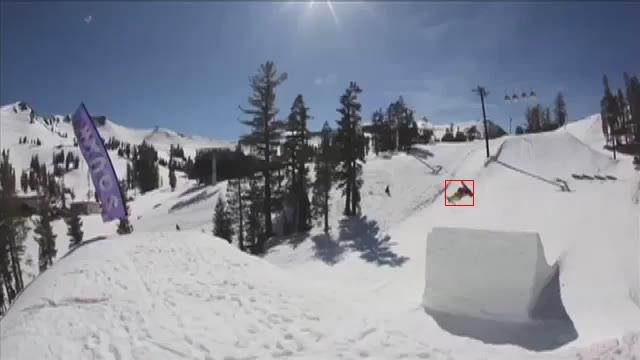
\includegraphics[width = 2.5in]{Skiing-0001}} \\
\subfloat[frame = 31]{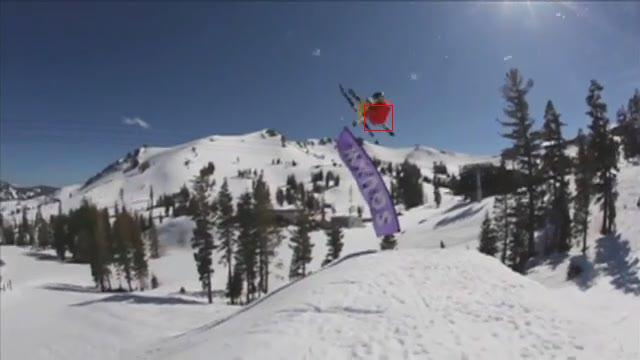
\includegraphics[width = 2.5in]{Skiing-0031}} \\
\subfloat[frame = 32]{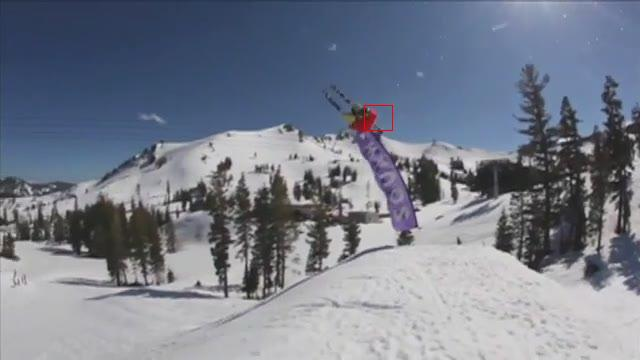
\includegraphics[width = 2.5in]{Skiing-0032}} \\
\end{tabular}
\centering
\caption{A video tracking sequence showing the tracking algorithm failing to account for changes in scale. Notice that by frame 32, the target object had grown so much that the tracking algorithm no longer recognized it.}
\label{fig:scaling2}
\end{figure}

\subsection{Miscellaneous Results}
Other than those tests already mentioned, we tested our algorithm on several other videos from the testing dataset. 
Some of these results are shown in the figures below and can also be seen on our GitHub page at \verb!https://github.com/msu-ml/16spr_cao_gonzales_hoffman/tree/master/results!.

\noindent{Note} that several figures appear \textit{after} the references section of the report.
Overall, we feel that our algorithm was able to perform well on video sequences that did not involve too much scale variation.
We believe that many of the primary problems the algorithm currently faces can be fixed through the future work we plan to implement.

\section{Conclusions and Future Work}
We were able to re-implement the results of Hong, et al.~\cite{hong2015online} in order to produce an object tracking algorithm for videos that worked surprisingly well overall.
This algorithm contributed to the field of object tracking in several ways.
The use of a CNN to extract features on the target object allowed us to overcome many of the traditional problems in object tracking, such as some lighting variations and object rotation.
The use of an online SVM on top of the CNN then allowed the algorithm to learn the representation of a specific object at runtime, improving tracking performance. 
We did run into some problems, such as the prior causing the tracker to lose fast moving objects and scale variations causing the tracker to lose objects moving too much towards or away from the camera.
However, we were able to circumvent some of these problems (e.g. removing the prior) and came up with plans for future work to solve some of the other problems (e.g. dealing with scale variations).
While our algorithm did not perform as well qualitatively as the results provided by Hong, et al., we recognize that the authors of that paper may have not included in their paper all of the optimizations they used for their algorithm, and they likely had a larger amount of time to fine tune the algorithm to the Tracking Benchmark v1.0 dataset.
They were also able to use the pre-trained \textit{R-CNN} in their algorithm, which is available in Caffe but not MatConvNet, and this may have caused significant differences in our results.

We learned many important aspects of object tracking while working on this project.
First off, we learned how to use a pre-trained CNN to create target-specific saliency maps in order to localize a target.
We found this a very interesting, ingenious way to use a CNN in object tracking.
This project also gave us experience implementing the results of someone else's paper and learning to interpret/discover the many parts of an algorithm that are not made clear in a paper.
During this project, we also had a hands-on experience dealing with many of the challenges involved in video tracking, such as scale variation, occlusions, deformations, fast motion, and object rotation.
If not accounted for, these challenges can absolutely devastate a tracking algorithm in only a few frames.
While this algorithm was able to handle many of these challenges, it could not handle all of them which led us to think deeper into how these challenges can be overcome.

In the future, we are hoping to continue modifying this algorithm and improving it to work in more situations.
One of the most obvious problems inherent in the algorithm that needs to be addressed is that of scale variation.
This algorithm currently assumes that the bounding box around an object can stay the same size throughout all the video frames.
However, this assumption proves to be false in far too many circumstances.
Therefore, we plan to modify our algorithm so that when we generate candidate sample patches, we will generate some that are smaller and some that are larger than the current bounding box size.
This would allow the bounding box to grow or shrink as needed.
We also noticed that if the algorithm does a poor job at classifying the target for several frames in a row, our current SVM training algorithm will begin training on these mistakes, leading to more mistakes in the future.
Occasionally, this causes no positive samples to be found in a frame. Currently, in this situation, we just set the bounding box to be the same as that in the previous frame and then continue to the next frame.
In the future, we plan to modify the SVM in a few ways to help account for this.
First, if no positive samples are found, we plan to then back-propagate most or all of the samples through the CNN, with the hope that the target object, although not found by the SVM, will be found in some of these samples and will be found by the target posterior.
Then we could retrain the SVM including this new target location.
Also, we plan to decrease the amount of allowed overlap between the positive sample fed to the SVM and the negative samples fed to the SVM so that there is less likelihood it will be told that a sample including large parts of the target is a negative sample during training.
Thirdly, we also wish to modify the SVM so that it is a truly incremental, online SVM; currently, we have to retrain the SVM on \textit{all} the training data every time we wish to train it.
Because of this, we had to significantly decrease the amount of training samples we feed the SVM to decrease the amount of time it takes to train.
If we could implement an incremental, online SVM, then each time we train it we would only feed it the \textit{new} training samples, i.e. those from the previous frame.
This would allow it to train on a much larger set of training samples and become much more accurate, we hope.
Other than these updates, we have some other future work planned as well.
For instance, we may turn our main program file into a function to make it easier to call, may add an option to track multiple objects, and may investigate tracking objects in spectra other than the visible light spectrum, such as in thermal videos.

\section{Work Distribution among Authors}
This section outlines how the work was distributed between the two authors of this report. 

\subsection{Aaron Gonzales}
\textit{Aaron Gonzales} was primarily responsible for generating the candidate sample patches, for using an SVM to find the target-specific features from the sample features, and training the online SVM.
He also researched the related work and was the primary contributor towards creating the final project presentation.

\subsection{Steven Hoffman}
\textit{Steven Hoffman} was primarily responsible for writing the skeleton code for the overall tracking algorithm, passing samples through the CNN to get the sample features, back-propagating the target-specific features through the CNN to create a target-specific saliency map, computing the generative model, and finding the target posterior.
He also was the primary contributor towards creating the final project report.

\subsection{Both Authors}
\textit{Both authors} worked together to write up the various project reports, to give the final presentation, and to run the code on various testing sequences (i.e. videos).

\bibliography{proj-report}
\bibliographystyle{unsrt}
\end{document}
